\section{Facts}
\label{sec:facts}

A \textbf{fact} is the smallest unit of information in an XBRL report. 
According to the XBRL glossary, a fact is a term used to describe an individual piece of financial or business information within an XBRL instance document\cite{xbrl_glossary}.
% The word "Fact" is a term used to describe an individual piece of financial of business information within an XBRL instance document\cite{xbrl_glossary}.
This section aims to represent facts and its supporting concepts in a way that is in line with the OIM.

% Lets consider a simplified example involving a financial report of Microsoft Corporation for the fiscal year 2022.
% Microsoft's annual report can be found on the company's website\footnote{https://www.microsoft.com/investor/reports/ar22/index.html}.
% It contains a lot of information about the company's financial situation, as well as information about the company's business activities.
% For this example, we will only consider the company's revenue for the fiscal year 2022.
% Microsoft chose to report this information as follows:
% Let's examine a simplified case focusing on the financial report of Microsoft Corporation for the fiscal year 2022.
Consider a simplified example involving Microsoft Corporation's financial report for the fiscal year 2022.
Microsoft's annual report is accessible on the company's investors page\footnote{https://www.microsoft.com/investor/reports/ar22/index.html}.
This document provides extensive details about Microsoft's financial health and its business operations.
In this scenario, we will solely focus on the company's revenue for the fiscal year 2022,
as reported by Microsoft in the following manner:

\begin{figure}[H]
    \centering
    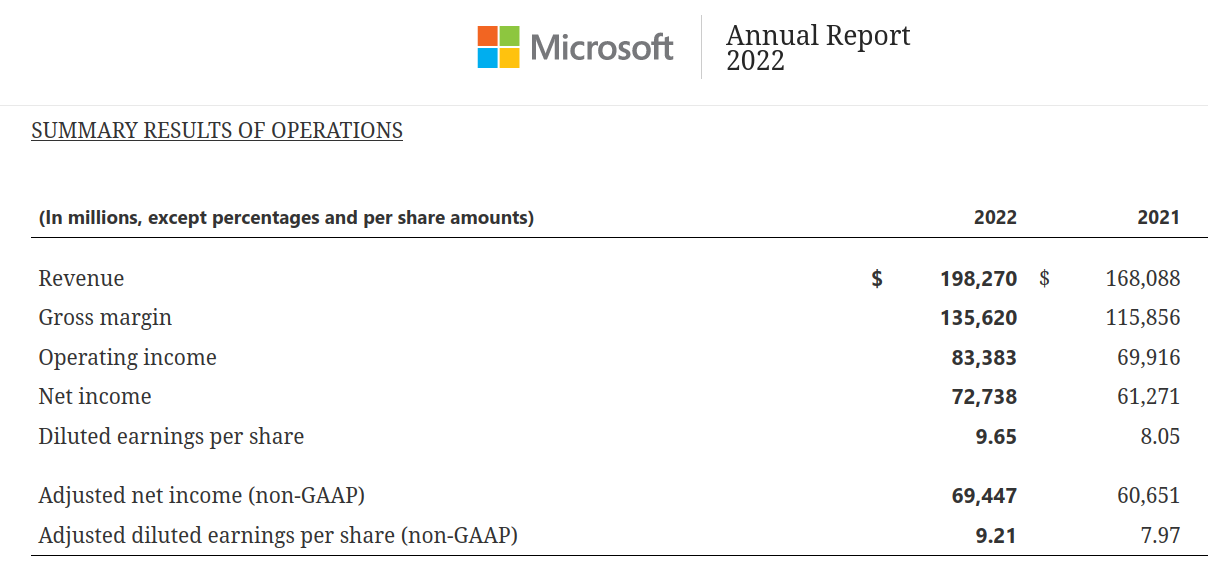
\includegraphics[width=0.75\textwidth]{images/microsoft_annual_report_2022.png}
\caption{Microsoft's summary results of operations for the fiscal year 2021 and 2022\cite{microsoft2022ar}}
    \label{fig:microsoft_annual_report_2022}
\end{figure}

% This table contains multiple facts about Microsoft for both fiscal years 2021 and 2022, as seen by the horizontal axis.
% The vertical axis describes what is being reported. The "what is being reported" part is called the \textbf{concept} of a fact.
% It reports the values for the concepts "Revenue", "Gross margin", "Operating income", \dots for both fiscal years.
% In summary, the table contains 14 facts across 7 concepts for 2 fiscal years.

% For now, let us focus on the top left fact, which reports the company's revenue for the fiscal year 2022.
% In XBRL, a corresponding fact would be represented as follows:
This table displays multiple facts about Microsoft for the fiscal years 2021 and 2022, as indicated by the horizontal axis.
The vertical axis outlines the subjects of these facts, with the term \textbf{concept} used to describe what each fact reports.
Values for concepts such as "Revenue", "Gross Margin", "Operating Income", etc., are presented for both fiscal years.
To summarize, the table showcases 14 facts across 7 concepts for two fiscal years.

For the moment, our attention will be on the top left fact, which details the company's revenue for the fiscal year 2022.
In XBRL terminology, this specific fact would be represented in the following way:

\begin{itemize}
    \item \textbf{Concept:} Revenue
    \item \textbf{Entity:} Microsoft Corporation
    \item \textbf{Period:} from 2022-04-01 to 2023-03-31 \footnote{Refers to the fiscal year 2022, which starts on April 1, 2022, and ends on March 31, 2023}
    \item \textbf{Unit:} USD
    \item \textbf{Value:} 198'270'000 \footnote{https://www.microsoft.com/investor/reports/ar22/index.html}
\end{itemize}

In this example:

\begin{itemize}
    \item The \textbf{concept} refers \textit{what} is being reported. 
    In this case, "Revenue" signifies the fact pertains to the company's revenue figures.
    \item The \textbf{entity} points to \textit{who} is reporting. 
    For our example, the entity is "Microsoft Corporation".
    Though implicitly understood from Microsoft's annual report,
    the entity of a fact must be explicitly mentioned in an XBRL report.
    \item The \textbf{period} specifies \textit{when} the information is being reported,
    defined here as the fiscal year 2022, as shown by the "2022" column heading.
    \item The \textbf{unit} clarifies \textit{how} the information is presented,
    with "USD" indicating the figures are in US dollars,
    marked by the dollar symbol \$ in the table.
    \item The \textbf{value} reveals \textit{how much} is being reported,
    with Microsoft's 2022 annual report stating the company's revenue for the fiscal year 2022 as approximately 198 billion US dollars.
\end{itemize}

% The concept, entity, period and unit of a fact are called its \textbf{aspects}. 
% If necessary, additional aspects can be defined for a fact. 
% These additional aspects are called \textbf{dimensions} and will be covered in section \ref{sec:hypercubes}
% The aspects that are not dimensions are called \textbf{core aspects}. 
% Even though the name suggests otherwise, core aspects are not all mandatory for a fact.
% The only mandatory core aspect is the concept.

The concept, entity, period, and unit associated with a fact are referred to as its \textbf{aspects}.
If necessary, facts can be further detailed through \textbf{dimensions}, which are additional aspects that will be elaborated on in section \ref{sec:hypercubes}.
Aspects that are not dimensions are known as \textbf{core aspects}.
Contrary to what the term might imply, not all core aspects are compulsory for a fact to have.
The only mandatory core aspect is the concept.